\section{Map-Reduce Pipelines}
Large-scale data-parallel computation is increasingly important.  Technologies such as MapReduce provide useful functional programming constructs for parallelizing compute-intensive jobs.  However, debugging data-parallel programs remains difficult, particularly with regard to errors in giga-, tera-, and peta-scale inputs.  For example, the presence of a single unexpected zero value can dramatically alter the result of many mathematical programs.  Finding and correcting these errors, preferably automatically, is an important step in making large-scale computation more robust.

\begin{figure*}[t]
	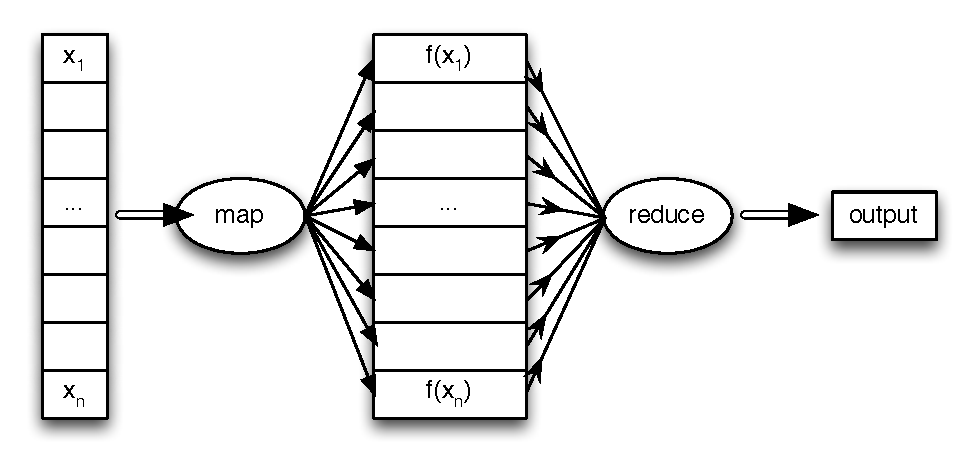
\includegraphics[width=2.5in]{images/mapreduce}
  % \hspace{30px}
  \hfill
	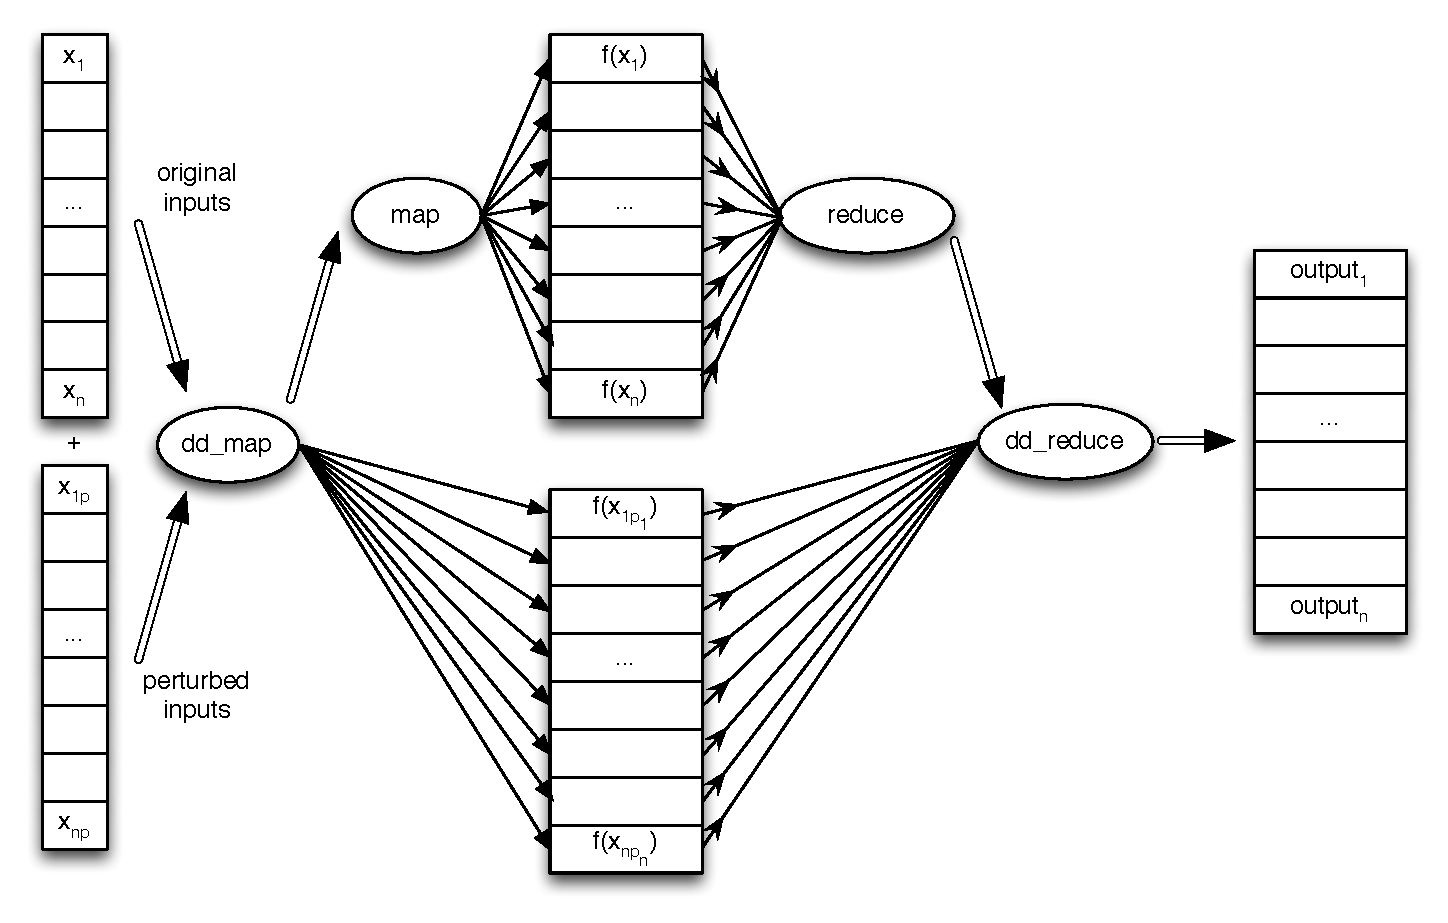
\includegraphics[width=3.25in]{images/mapreduce_dd}
	\caption{
		On the left, a typical MapReduce job.  On the right, a data-debug-augmented MapReduce job.  Each additional output is a version of the computation with the unusually-impactful values automatically excluded.\label{fig:mapreduce_pipeline}
	}
\end{figure*}

MapReduce and Hadoop jobs are low-level programming idioms, but frameworks like FlumeJava (and by extension, its Hadoop dual, Crunch) allow multi-stage MapReduce programs to be represented by higher-level programming constructs~\cite{pldi:flumejava}.  These constructs allow the runtime to determine a program dependency graph.  This higher-level representation gives the runtime global information that facilitates automatic performance-enhancing program transformations, such as reordering of functions in the program call graph to increase parallelism.

Data-parallel programs share many of the same properties that make data-debugging a useful technique in spreadsheets.  The input to the mapper stage of a MapReduce problem is a large, homogenous vector amenable to the same kind of input perturbation that \checkcell{} uses.  A key property of the computation kernel in a MapReduce job is that code be shared-nothing and re-entrant, thus data-debugging, which often needs to recompute certain portions of the call graph, can be inserted into a portion of a MapReduce job without affecting the semantics of the original program.

As with \checkcell, data-debugging functions can transparently augment a FlumeJava program.  The tradeoff, which we seek to minimize, is a small performance penalty for the additional robustness data-debugging provides. Data-debugging techniques can be piggybacked on a high-level representation so that impact analysis can take advantage of underutilized parallelism to minimize the performance impact of our technique.

Large-scale data-debugging requires at least two kinds of program transformations to be feasible.  First, a data-debugging-enhanced library like FlumeJava would augment the map stage with perturbed input values to be computed in parallel, and the reducer function would be augmented with the impact computation.  Our implementation of \checkcell relies on Microsoft Excel's ability to recognize when partial recomputation of the dependency graph is possible, for efficiency purposes.  Thus, second, a data-debugging-enhanced FlumeJava runtime would both need to recognize when an impact calculation may be performed for only a subset of the program dependency graph and when the dependency analysis itself contains overlapping subproblems whose solutions should be shared for performance speedups.

Once impact scores are known for a set of MapReduce program inputs, the data-debug runtime can be instructed to re-run the computation with the unusually-impactful inputs either removed or replaced with user-specfied values.  The degree of unusualness, in terms of standard deviations from the norm, may be used to control the degree of \emph{input trimming} performed on the MapReduce input vector.  Again, a high-level representation of the program graph allows this recomputation to be performed for the minimum cost possible.